\chapter{Tecnologías utilizadas}

\section{Visión general}

En esta sección se presentan las diferentes tecnologías que se han utilizado para el desarrollo del proyecto. Las principales tecnologías usado son las siguientes:

\section{Microsoft Azure}

Microsoft Azure\cite{Azure} es una plataforma e infraestructura de cloud computing creada por Microsoft para desarrollar, desplegar y gestionar aplicaciones y servicios a través de una red global de data centers gestionados por Microsoft.
Proporciona servicios tanto \acrshort{paas} como \acrshort{iaas} y soporta una multitud de lenguajes de programación, herramientas e infraestructuras, ya sean propias de Microsoft o de terceros.

\begin{figure}[!htbp]
	\centering
	
\includegraphics[scale=1.2]{fig/microsoft_azure}
	\caption{Logotipo de Microsoft Azure}
\end{figure}

Los servicios de Azure utilizados en este proyecto son los siguientes:
\begin{itemize}
	\item Creación y hospedaje de una aplicación web
	\item Creación y hospedaje de un servidor \acrshort{sql}
	\item Creación y hospedaje de una \acrshort{bd} \acrshort{sql}
\end{itemize}

\subsection{Razón de uso}

\begin{itemize}
	\item Al ser ambos productos de Microsoft, la integración entre Microsoft Azure y Microsoft Visual Studio Enterpise 2015 es inmejorable, haciendo que el despliegue de aplicaciones sea fácil y rápido.
	\item Familiaridad del equipo con la plataforma.
	\item Al ser un servicio ofrecido por un gigante de las tecnologías de información como Microsoft, se puede esperar que el servicio será seguro y fiable y cuente con un buen soporte en el caso de incidencias.

\end{itemize}

\section{Microsoft Cognitive Services}

Microsoft Cognitive Services\cite{Oxford} (anteriormente Project Oxford) es un conjunto de \acrshort{api}s, \acrshort{sdk}s y servicios disponibles a los desarrolladores para que hagan sus aplicaciones más inteligentes, interactivas y accesibles. Microsoft Cognitive Services expande el abanico ya existente de APIs de machine learning creadas por Microsoft y permite a los desarrolladores añadir características inteligentes de forma fácil, tales como reconocimiento de voz, facial, emoción y visión, así como comprensión de lenguaje natural.

\subsection{Razón de uso}

\begin{itemize}
	\item Existencia de pruebas gratuitas
	\item Documentación extensa, clara y concisa.

\end{itemize}

\section{Universal Windows Platform}

La \acrfull{uwp}\cite{UWP} es una arquitectura de aplicación homogénea creada por Microsoft y introducida por primera vez en Windows 10, el propósito de esta plataforma es ayudar a desarrollar aplicaciones de estilo Metro que puedan ejecutarse en cualquier dispositivo Windows 10 sin necesidad de ser reescritas, soporta el desarrollo de aplicaciones de Windows usando C++, C\#, \acrshort{vb.net} o \acrshort{xaml}. La API está implementada en C++ y soportada en C++, \acrshort{vb.net}, C\#, F\# y \acrfull{js}. Diseñada como una extensión de la plataforma Windows Runtime introducida en Windows Server 2012 y Windows 8, \acrshort{uwp} permite a los desarrolladores crear aplicaciones que puedan, potencialmente, ejecutarse en múltiples tipos de dispositivos.

\begin{figure}[!htbp]
	\centering
	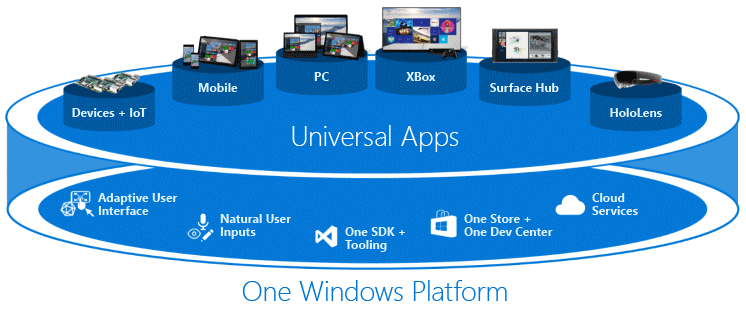
\includegraphics[scale=0.7]{fig/uwp_representation}
	\caption{Representación de \acrshort{uwp}}
\end{figure}

\FloatBarrier

\subsection{Razón de uso}

La Plataforma Universal Windows proporciona recursos como Windows.Media.Capture o Windows.Devices.Geolocation, que son utilizados en este proyecto, \acrshort{uwp} incluye muchas librerías que permiten a un programador acceder a los recursos del sistema de una forma estandarizada sin necesidad de preocuparse de que hardware se use, con MediaCapture, una aplicación \acrshort{uwp} es capaz de usar el mismo código para acceder a una cámara \acrshort{usb} de hace 10 años y una que acaba de salir de la fábrica, siempre y cuando el sistema tenga los drivers adecuados, se da el mismo caso con la librería Geolocation, no siendo necesario hacer ninguna consideración sobre que hardware debe tener el dispositivo, independientemente de si el dispositivo en el que el código se ejecuta tenga \acrshort{gps}, \acrshort{wifi} o una conexión por cable a internet, el código subyacente determinará la posición del dispositivo de la manera que estime conveniente de acuerdo con la petición que se le ha realizado (si se requiere alta precisión, o no), esto hace que la codificación de funciones complejas que hace años habría llevado una gran cantidad de tiempo hoy en día se pueda hacer en menos de una hora.

\lstinputlisting[frame=single, caption=Código para manejo de WebCam]{content/code/mediacapture.cs}
\lstinputlisting[frame=single, caption=como obtener la localización del dispositivo]{content/code/geolocation.cs}

\section{ASP.NET}

ASP.NET\cite{asp.net} es una infraestructura open-source de aplicaciones web server-side diseñada para el desarrollo web de páginas web dinámicas, fue originalmente desarrollada exclusivamente por Microsoft, es ideal para crear paginas basadas en los estándares \acrshort{html}5, \acrshort{css}3 y \acrfull{js} e incluye tres maneras distintas de trabajar:

\begin{itemize}

\item \textbf{ASP.NET Web Forms:} usa controles y un modelo de eventos para un desarrollo basado en componentes

\item \textbf{ASP.NET \acrshort{mvc}:} \acrshort{mvc} valora la separacion de conceptos y permite usar la metodología \acrshort{tdd} de una forma mas facil

\item \textbf{ASP.NET Web Pages:} Web Pages prefiere un modelo de página unica que mezcla codigo y marcado \acrshort{html}.

\end{itemize}

Todas estas técnicas se pueden mezclar en la misma aplicación al ser todo ASP.NET

\begin{figure}[!htbp]
	\centering
	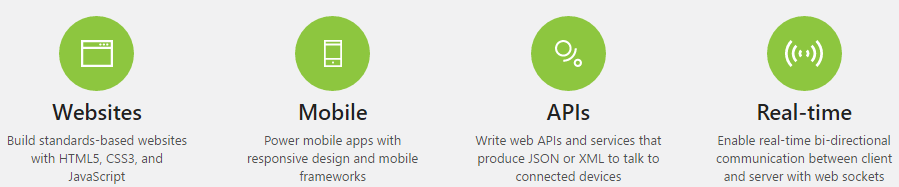
\includegraphics[scale=0.6]{fig/asp-net_highlights}
	\caption{Aspectos destacados de ASP.NET}
\end{figure}

ASP.NET incluye la ASP.NET Web \acrshort{api} para crear servicios \acrshort{rest}-ful de calidad que devuelvan \acrshort{json}, \acrshort{xml} o cualquier tipo de contenido que soporte la web, las ASP.NET Web \acrshort{api}s pueden proveer servicios de datos a aplicaciones móviles como las de Windows Phone, iPhone, Android y más, también pueden ser usadas en cualquier tipo de aplicación ASP.NET, ya sea Web Forms, \acrshort{mvc} o Web Pages.

ASP.NET SignalR es una librería para desarrolladores de ASP.NET que convierten la comunicación bi-direccional de cliente y servidor en tiempo real en realidad, SignalR permite el uso de nuevos estándares como Web Sockets manteniendo la compatibilidad con exploradores más antiguos, puede soportar clientes \acrfull{js}, al igual que clientes en Android, iPhones y todos los clientes basados en C# como Windows Phone y Windows 8.

ASP.NET puede usarse para crear aplicaciones móviles con \acrshort{rwd} gracias a tener Twitter Bootstrap incorporado desde Visual Studio 2013, se puede usar cualquier framework \acrshort{css} o sistemas como JQuery Mobile o Sencha.

Stack Overflow\cite{StackOverflow} usa ASP.NET \acrshort{mvc} para su página junto a \acrshort{sql} Server y otras tecnologías de Microsoft

En este caso en concreto se ha utilizado ASP.NET \acrshort{mvc}, radicalmente distinto a ASP.NET Web Forms y que usa el patrón \acrfull{mvc}.

\begin{figure}[!htbp]
	\centering
	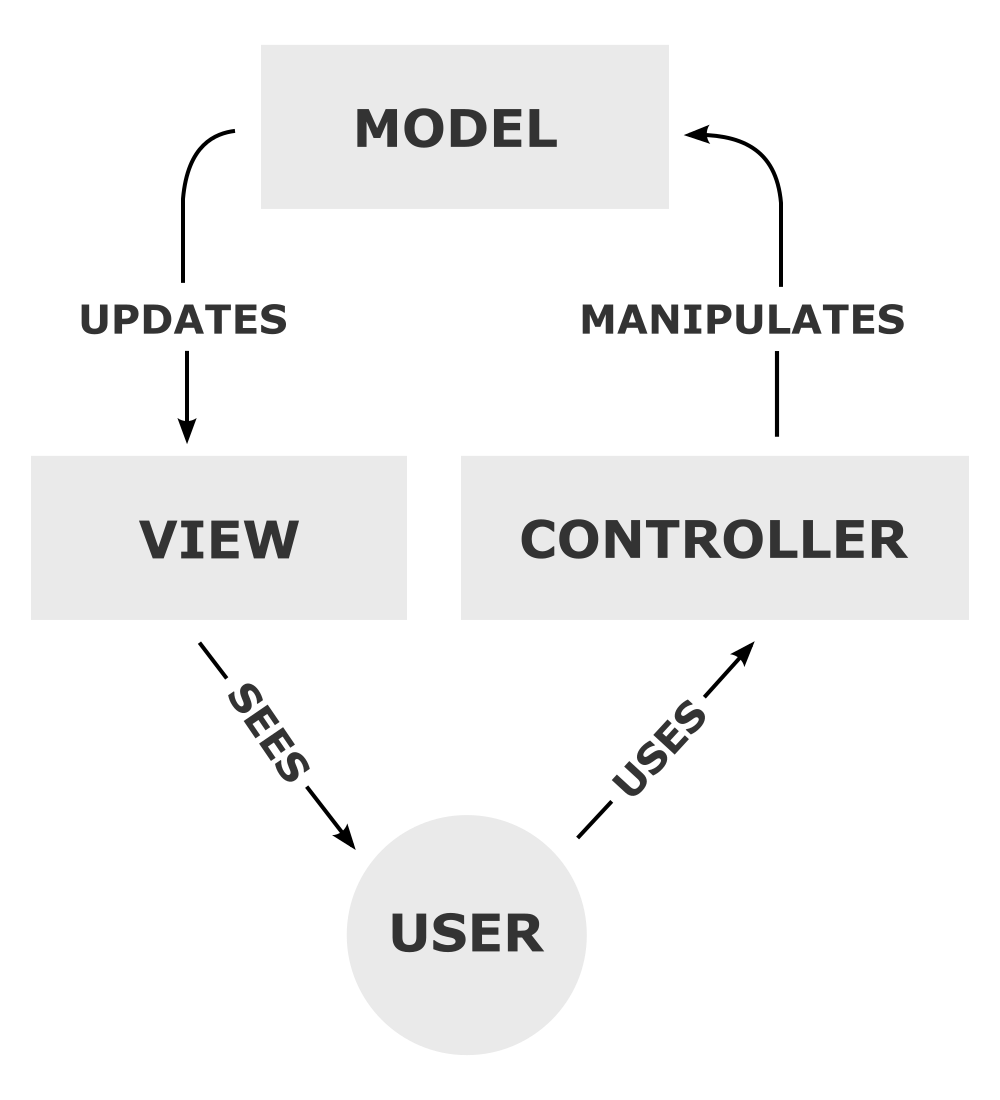
\includegraphics[scale=0.50]{fig/mvc_pattern}
	\caption{Representación del patrón \acrshort{mvc}}
\end{figure}

\subsection{ASP.NET Razor}

Razor es una sintaxis de programación de ASP.NET usada para crear páginas web dinámicas con \acrshort{vb.net} o C#, Razor fue lanzado para Visual Studio 2010 en enero de 2011 como parte de ASP.NET \acrshort{mvc} 3 y el set de herramientas WebMatrix.

\lstinputlisting[frame=single, caption=Ejemplo de una vista en ASP.NET Razor]{content/code/externalloginview.cshtml}

\subsection{Razón de uso}

\begin{itemize}
	\item Una gran variedad de plantillas de calidad para desarrollar aplicaciones web rápidamente, así como placeholders para autenticación con servicios externos ya incluidos en ellas.
	\item Extensa documentación y tutoriales creados por Microsoft.
	\item Bootstrap integrado junto con la mayoría de las plantillas.

\end{itemize}

\section{Application Insights}

\acrfull{ai}\cite{AI}, también denominado Visual Studio \acrfull{ai} es una herramienta de depuración de errores que permite detectar y diagnosticar errores en una aplicación web sin tener que conectar un debugger a la misma.

\begin{figure}[!htbp]
	\centering
	
\includegraphics[scale=0.50]{fig/applicationinsights_logo}
	\caption{Logotipo de \acrfull{ai}}
\end{figure}

Usado por clientes como Xerox\cite{Xerox}, \acrshort{ai} permite realizar un amplio análisis de una página o aplicación web en ejecución, pudiendo recabar datos sobre fallos del servidor (excepciones, peticiones fallidas, etc.) o rendimiento (tiempo de respuesta, número de peticiones), \acrshort{ai} utiliza Machine Learning para analizar constantemente una aplicación y determinar su funcionamiento normal, para así detectar comportamientos anómalos de manera más efectiva, permitiendo a los desarrolladores encontrar errores en su aplicación antes de que estos afecten el funcionamiento del código de forma significativa.

\subsection{Razón de uso}

Al no poder estar monitorizando el servidor desplegado en Azure para servir de fuente de datos al Smart Mirror todo el rato mediante la conexión de un debugger de Visual Studio a este, \acrshort{ai} ha sido una herramienta inestimable para diagnosticar problemas que no son evidentes en una primera ejecución del código y que solo aparecen bajo circunstancias especiales.

\section{Bootstrap}

Boostrap\cite{Bootstrap} es una infraestructura gratuita y de código abierto para uso en front-ends de sitios y aplicaciones web, contiene plantillas basadas en \acrshort{html} y \acrshort{css} para tipografías, formularios, botones, elementos de navegación y otros componentes de interfaz, además de extensiones \acrfull{js} opcionales, a diferencia de muchos otros frameworks, se limita únicamente al desarrollo de front-ends.

\begin{figure}[!htbp]
	\centering
	
\includegraphics[scale=0.50]{fig/bootstrap_logo}
	\caption{Logotipo de Bootstrap}
\end{figure}

Bootstrap, originalmente llamado Twitter Blueprint fue desarrollado por Mark Otto y Jacob Thornton en Twitter como una infraestructura para fomentar la consistencia entre varias herramientas internas. Antes de Bootstrap, el desarrollo de interfaces se realizaba haciendo uso de varias librerías, lo cual causaba inconsistencias y representaba un gran obstáculo para el mantenimiento.

\subsection{Razón de uso}

Aparte de estar incluido en las plantillas de ASP.NET, Bootstrap proporciona una manera fácil y rápida de diseñar e implementar páginas que usen \acrfull{rwd}, y que tengan un aspecto agradable para el usuario, aparte de una gran cantidad de código \acrfull{js} para asegurarse de que la interfaz es lo más fluida posible.

\section{Google APIs}

Google \acrshort{api}s\cite{GoogleAPIs} es un conjunto de \acrfull{api}s desarrolladas por Google que permiten comunicarse con Google Services e integrar soluciones en otros servicios como Google Search, Mail, Translate, Maps, o Calendar, dicha integración se realiza a menudo haciendo uso de OAuth 2.0, descrito en otro apartado de este capítulo.

Google ofrece librerías que permiten trabajar con Google \acrshort{api}s para múltiples lenguajes de programación como Java, \acrfull{js}, .NET, Objective-C, \acrshort{php} y Python, así como guías y ejemplos de código que permiten al desarrollador hacerse una idea de cómo trabajar con ellas rápidamente.

\subsection{Razón de uso}

Google proporciona acceso gratuito a sus \acrshort{api}s mientras que Microsoft requiere una licencia de desarrollo para su plataforma de \acrshort{api}s de Outlook, considerando además la popularidad de las cuentas Google frente a las cuentas de Outlook, resultaba más práctico hacer uso de los servicios de Google.

\section{OAuth}



\subsection{Razón de uso}

\section{OpenWeatherMap}

\subsection{Razón de uso}

\section{Raspberry Pi}

\subsection{Razón de uso}

\section{Entity Framework}

\subsection{Razón de uso}